
%% Template by Michal Forisek


\documentclass[12pt,a4paper]{report}
%\usepackage{slovak}
\usepackage[utf8]{inputenc}
\usepackage[IL2]{fontenc}
%\usepackage{a4wide}
\usepackage{tabularx}
\usepackage{amsfonts}
\usepackage{amssymb}
\usepackage{amsmath}
\usepackage{amsthm}
\usepackage{mathtools}
%\usepackage{breqn} % messes up biblatex and \log_2
%\usepackage{epsfig}
\usepackage{color}
\usepackage{mathrsfs}
\usepackage{verbatim}
\usepackage{fancyvrb}
\usepackage{float}
\usepackage{longtable}
\usepackage{listings}
\usepackage{graphicx}
\usepackage{changepage}
\usepackage{caption}
\usepackage{subcaption}
\usepackage{multirow}
\usepackage{paralist}
\usepackage{pdfpages}
\usepackage{tikz}
\usepackage{pgfplots}
\usepackage{gnuplot-lua-tikz}
\usetikzlibrary{arrows}
\usetikzlibrary{positioning}
\usetikzlibrary{shapes}
\usetikzlibrary{calc}
\usetikzlibrary{decorations.pathreplacing}
\usetikzlibrary{backgrounds}
\usetikzlibrary{fit}
\usepackage[style=alphabetic,maxbibnames=47,backend=biber]{biblatex}
% vim: set fdm=marker:
%% Original by Michal Forisek

%% zakladne definicie
\newcommand{\quoteme}[1]{\clqq#1\crqq}
\def\todo#1{[{\color{red} TODO:} {\bf  #1}]}
\def\fixme#1{[{\color{red} FIXME:} {\bf  #1}]}
\def\verify#1{\todo{verify: #1}}

\def\problem#1{\textsc{#1}}
\def\graphcol#1#2{\problem{GraphColoring(#1, #2)}}
\def\sgkh#1{\problem{$#1$-SGKH}}
\def\sguh#1{\problem{$#1$-SGUH}}

\def\phi{\varphi}
\def\xor{\oplus}
\def\concat{\|}
%\def\inr{\in_{R}}
\def\toa #1 {\overset{#1}{\rightarrow}}
\def\inr{\overset{\$}{\leftarrow}}
\def\assign{\leftarrow}
\def\send{\rightarrow}
\def\isomorph{\cong}
\def\nsd{NSD}
\def\union{\cup}
\newcommand{\unit}[1]{\ensuremath{\, \mathrm{#1}}}
\newcommand{\mset}[1]{\ensuremath{\mathbb{#1}}}
\newcommand{\Zn}[1]{\ensuremath{\mset{Z}_{#1}}}
\DeclareMathOperator{\dlog}{dlog}
\def\code#1{\lstinline@#1@}
\def\classname#1{{\tt #1}}

\def\compactlist{
  \setlength{\itemsep}{1pt}
  \setlength{\parskip}{0pt}
  \setlength{\parsep}{0pt}
}

%% Labely s predefinovanym asociovanym textom
\makeatletter
\def\textlabel#1#2{%
  \@bsphack\begingroup
  \protected@write\@auxout{}{\string\newlabel{#2}{{\@currentlabel}{\thepage}{#1}{\@currentHref}{}}}%
  \endgroup\@esphack
}%
\makeatother


%%% original od Misofa:
%% {{{

\catcode`\@=11

\def\R{\mset{R}}
\def\cent{{c\kern-0.3em|\kern0.1em}}
\def\N{\mset{N}}

\let\eps=\varepsilon

\def\relupdown#1#2#3{\mathrel{\mathop{#1}\limits^{#2}_{#3}} }

\let\then=\Rightarrow
\let\neht=\Leftarrow

\def\krok#1{\relupdown{\Longrightarrow}{}{#1}}
\def\thenrm{\relupdown{\Longrightarrow}{}{rm}}

\def\bicik{\upharpoonright}
\def\B{{\mathbf B}}
\def\kodTS#1{{\tt <}#1{\tt >}}

\newtheorem{definicia}{Definícia}[section]
\newtheorem{HLPpoznamka}{Poznámka}[section]
\newtheorem{HLPpriklad}{Príklad}[section]
\newtheorem{HLPcvicenie}[HLPpriklad]{Cvičenie}
\newtheorem{zadanie}{Úloha}[section]
\newenvironment{poznamka}{\begin{HLPpoznamka}\rm}{\end{HLPpoznamka}}
\newenvironment{priklad}{\begin{HLPpriklad}\rm}{\end{HLPpriklad}}
\newenvironment{cvicenie}{\begin{HLPcvicenie}\rm}{\end{HLPcvicenie}}
\newtheorem{veta}{Veta}[section]
\newtheorem{lema}[veta]{Lema}
\newtheorem{dosledok}[veta]{Dôsledok}
\newtheorem{teza}[veta]{Téza}
% \newtheorem{dokaz}{Dôkaz}[section]

\newtheorem{definition}{Definition}[chapter]
\newtheorem{theorem}[definition]{Theorem}
\newtheorem{lemma}[definition]{Lemma}
\newtheorem{corollary}[definition]{Corollary}
\newtheorem{observation}[definition]{Observation}

\long\def\odsadene#1{
\leftskip=\parindent
\parindent=0pt
\vskip-5pt

\parskip=5pt
#1
\parskip=0pt

\parindent=\leftskip
\leftskip=0pt

} % end \odsadene




%%%%%%%%%%% PROSTREDIE PRE PISANIE KOMENTAROV

%\newenvironment{komentar}{%
%\vskip\baselineskip
%\tabularx{0.95\textwidth}{|X|}
%\sl
%}
%{\endtabularx
%\vskip\baselineskip
%}

\newenvironment{komentar}{%
\vskip\baselineskip\noindent
\tabularx{\textwidth}{>{\hsize=.2\hsize}X>{\hsize=1.8\hsize}X}
\sl ~ & \sl
}
{\endtabularx
\vskip\baselineskip
}

%\newenvironment{komentar}{%
%\vskip\baselineskip
%\trivlist\vspace{-4pt}\raggedleft\item\relax\tabularx{0.9\textwidth}{X}\sl}
%{\endtabularx\vspace{-4pt}\endtrivlist
%\vskip\baselineskip
%}

\newenvironment{dokaz}{\trivlist
  \item[\hskip \labelsep{\bfseries Dôkaz.}]}{\endtrivlist}
  
%\newenvironment{dokaz}{%
%\vskip\baselineskip\noindent
%\tabularx{\textwidth}{||X||}
%\sl
%}
%{\endtabularx
%\vskip\baselineskip
%}

%%%%%%%%%%% PROSTREDIE PRE MOJE ITEMIZE 

\newenvironment{myitemize}{%
\begin{itemize}
\itemsep-3pt
}
{\end{itemize}
}

%%%%%%%%%%% MATICKE MAKRA

\font\tenrm=csr10

\def\eps{\varepsilon}
% \def\R{{\mathbb R}}
\def\lvec#1{\overrightarrow{#1}}
\def\uhol{{\measuredangle}}
\def\then{\Rightarrow}
% \def\lg{{\rm lg}}
\def\lg{\log_2}
%\def\div{\mathbin{\rm div}}
\def\div{{\rm div}}
\DeclarePairedDelimiter{\ceil}{\lceil}{\rceil}
\DeclarePairedDelimiter{\floor}{\lfloor}{\rfloor}
\DeclarePairedDelimiter{\paren}{(}{)}

%%%%%%%%%%% PDF

%\newif\ifpdf
%\ifx\pdfoutput\undefined
%  \pdffalse
%\else
%  \pdfoutput=1 \pdftrue
%\fi

%%%%%%%%%%% OBRAZKY 

\newcommand{\myincludegraphics}[2][]{\includegraphics[#1]{images/#2}}

%%%%%%%%%%% SLOVNICEK

\openout2=\jobname.slo

\newcommand{\definuj}[3][]{%
\def\tmpvoid{}\def\tmpfirst{#1}%
\ifx\tmpvoid\tmpfirst%
  {\sl #2}\label{definicia:#2}\write2{#2 & #3 & \pageref{definicia:#2} \cr}%
\else%
  {\sl #2}\label{definicia:#2}\write2{#1 & #3 & \pageref{definicia:#2} \cr}%
\fi}

\newcommand{\definujsilent}[2]{%
\label{definicia:#1}\write2{#1 & #2 & \pageref{definicia:#1} \cr}%
}

\newcommand\myglossary{
  \immediate\closeout2 
  %\if@twocolumn\@restonecoltrue\onecolumn\else\@restonecolfalse\fi
  \chapter{Slovníček pojmov}
  \begin{tabular}{|l|l|r|}
  \hline
  {\bfseries slovenský pojem} & {\bfseries anglický preklad} & {\bfseries str.} \\ 
  \hline
  \InputIfFileExists{\jobname.srs}{}{~ & ~ & ~ \\}
  \hline
  \end{tabular}
  %\if@restonecol\twocolumn\fi
}

%%%%%%%%%%% UVODZOVKY

\catcode`\"=13
\def "{\begingroup\clqq\def "{\endgroup\crqq}}
\def\dospecials{\do\ \do\\\do\{\do\}\do\$\do\&%
  \do\#\do\^\do\^^K\do\_\do\^^A\do\%\do\~\do\"}

%%%%%%%%%%% DANGER BENDS 

\font\manual=manfnt % font used for the METAFONT logo, etc.
\def\dbend{{\manual\char127}} % dangerous bend sign

\newlength{\bendwidth}   \settowidth{\bendwidth}{\dbend}    \newlength{\hangwidth}

\def\hangone{%
  \hangwidth=\bendwidth%
  \advance\hangwidth 5pt%
  \hangindent\hangwidth%
}
\def\hangtwo{%
  \hangwidth=\bendwidth%
  \multiply\hangwidth 2%
  \advance\hangwidth 6pt% 
  \hangindent\hangwidth%
}

\def\medbreak{\par\ifdim\lastskip<\medskipamount \removelastskip\penalty-100\medskip\fi}
\let\endgraf=\par

\def\d@nger{\medbreak\begingroup\clubpenalty=10000
%\def\d@nger{\begingroup\clubpenalty=10000
%  \def\par{\endgraf\endgroup\medbreak} \noindent\hangone\hangafter=-2
  \def\par{\endgraf\endgroup} \noindent\hangone\hangafter=-2
  \hbox to0pt{\hskip-\hangindent\dbend\hfill}}
\outer\def\danger{\d@nger}

\def\dd@nger{\medbreak\begingroup\clubpenalty=10000
%  \def\par{\endgraf\endgroup\medbreak} \noindent\hangtwo\hangafter=-2
  \def\par{\endgraf\endgroup} \noindent\hangtwo\hangafter=-2
  \hbox to0pt{\hskip-\hangindent\dbend\kern1pt\dbend\hfill}}
\outer\def\ddanger{\dd@nger}

\def\enddanger{\endgraf\endgroup} % omits the \medbreak
\def\enddangerhop{\endgraf\endgroup\medbreak}




\def\@nakedcite#1#2{{#1\if@tempswa , #2\fi}}
\DeclareRobustCommand\nakedcite{%
  \@ifnextchar [{\@tempswatrue\@nakedcitex}{\@tempswafalse\@nakedcitex[]}}
\def\@nakedcitex[#1]#2{%
  \let\@citea\@empty
  \@nakedcite{\@for\@citeb:=#2\do
    {\@citea\def\@citea{,\penalty\@m\ }%
     \edef\@citeb{\expandafter\@firstofone\@citeb\@empty}%
     \if@filesw\immediate\write\@auxout{\string\citation{\@citeb}}\fi
     \@ifundefined{b@\@citeb}{\mbox{\reset@font\bfseries ?}%
       \G@refundefinedtrue
       \@latex@warning
         {Citation `\@citeb' on page \thepage \space undefined}}%
       {\hbox{\csname b@\@citeb\endcsname}} }}{#1}}

\long\def\FIXME#1{
  \begin{center}
  \begin{minipage}{0.8\textwidth}
  {\bf FIXME:~}\sl #1
  \end{minipage}
  \end{center}
}


\catcode`\@=12
%% }}}


\def\author{Michal Petrucha}
\def\supervisor{RNDr. Michal Forišek, PhD.}
\def\titlea{Selected Topics}
\def\titleb{from Advice Complexity}
\def\title{\titlea{} \titleb}
\def\thesistype{Diploma thesis}
\def\year{2014}
\def\location{Bratislava}
\def\department{Department of Computer Science}
\def\studyprogram{Informatics}
\def\fieldnumber{2508}
\def\university{Comenius University in Bratislava}
\def\faculty{Faculty of Mathematics, Physics and Informatics}

\usepackage[hidelinks]{hyperref}

\addbibresource{literature.bib}

\newlength{\firstpagewidthinc}
% The length by which we want the first two pages wider:
\setlength{\firstpagewidthinc}{2cm}
\graphicspath{{img/}}
\linespread{1.3}

\lstset{numberstyle=none, basicstyle=\ttfamily,
showstringspaces=false, escapechar=\%, language=C++}

% TODO: Move the setup of packages into a separate file.

% Set up hyperref...
\hypersetup{
    pdfauthor = {\author},
    pdftitle = {\titlea{} \titleb},
    pdfkeywords = {online problem} {advice complexity} {approximation}
}

% TikZ setup for DPA and other graph figures.
\tikzstyle{vertex} = [circle, thick, draw, inner sep = 2]
\tikzstyle{full vertex} = [vertex, fill = black]
\tikzstyle{empty vertex} = [vertex, fill = white]
\tikzstyle{path vertex} = [full vertex]
\tikzstyle{query vertex} = [empty vertex]
\tikzstyle{edge} = [thick]
\tikzstyle{graph picture} = [scale = .6]
\tikzstyle{background highlight} = [rounded corners = 1ex,
                                    fill = black!30,
                                    transform shape,
                                    inner sep = .5em,
                                   ]

\begin{document}

\newlength{\firstpagewidth}
\setlength{\firstpagewidth}{\textwidth}
\addtolength{\firstpagewidth}{\firstpagewidthinc}

\pagenumbering{roman}

%%%%%%%%%%%%%%%%%% Obal %%%%%%%%%%%%%%%%%%
\thispagestyle{empty}
% Tu je kopa zakomentovanych riadkov, lebo Pastorovej sa z nejakeho dovodu
% nepaci v niektorych pracach, ze maju na obale logo, zatial co pri inych
% jej to vobec nevadi, tak nech je spokojna.
\begin{adjustwidth}{-0.5\firstpagewidthinc}{-0.5\firstpagewidthinc}
%\begin{minipage}{0.25\firstpagewidth}
%
\includegraphics[width=0.9\textwidth]{img/komlogo-new}
%\end{minipage}
%\begin{minipage}{0.69\firstpagewidth}
\begin{center}
\textsc{\university} \\
\textsc{\faculty} \\
\end{center}
%\end{minipage}

\bigskip
%3dc8ac68-0ab2-4817-b352-48b4038e9b46

\vfill
\begin{center}
\begin{minipage}{0.8\textwidth}
%\hrule
\bigskip\medskip
\centerline{\LARGE\sc\titlea}
\smallskip
\centerline{\LARGE\sc\titleb}
\smallskip
\centerline{\thesistype}
\end{minipage}
\end{center}
\vfill
\vfill
{\bf\year}
\hfill{\bf\author}
\end{adjustwidth}
\eject % EOP i


%%%%%%%%%%%%%%%%%% Titulna strana %%%%%%%%%%%%%%%%%%
\thispagestyle{empty}
\begin{adjustwidth}{-0.5\firstpagewidthinc}{-0.5\firstpagewidthinc}
\begin{minipage}{0.25\firstpagewidth}

\includegraphics[width=0.9\textwidth]{img/komlogo-new}
\end{minipage}
\begin{minipage}{0.69\firstpagewidth}
\begin{center}
\textsc{\university} \\
\textsc{\faculty} \\
\end{center}
\end{minipage}

\vfill
\begin{center}
\begin{minipage}{0.8\textwidth}
%\hrule
\bigskip\medskip
\centerline{\LARGE\sc\titlea}
\smallskip
\centerline{\LARGE\sc\titleb}
\smallskip
\centerline{\thesistype}
\bigskip
\bigskip
%\centerline{\large\sc \author}
\bigskip\bigskip
%\hrule
\end{minipage}
\end{center}
\vfill
\begin{tabular}{l l}
Study programme: & \studyprogram \\
Field of study: & \fieldnumber{} \studyprogram \\
Department: & \department \\
Supervisor: & \supervisor \\
\end{tabular}
\vfill
{\bf\location, \year}
\hfill{\bf\author}
\end{adjustwidth}

\eject % EOP i

%%%%%%%%%%%%%%%%%% Zadanie %%%%%%%%%%%%%%%%%%
%\thispagestyle{empty}

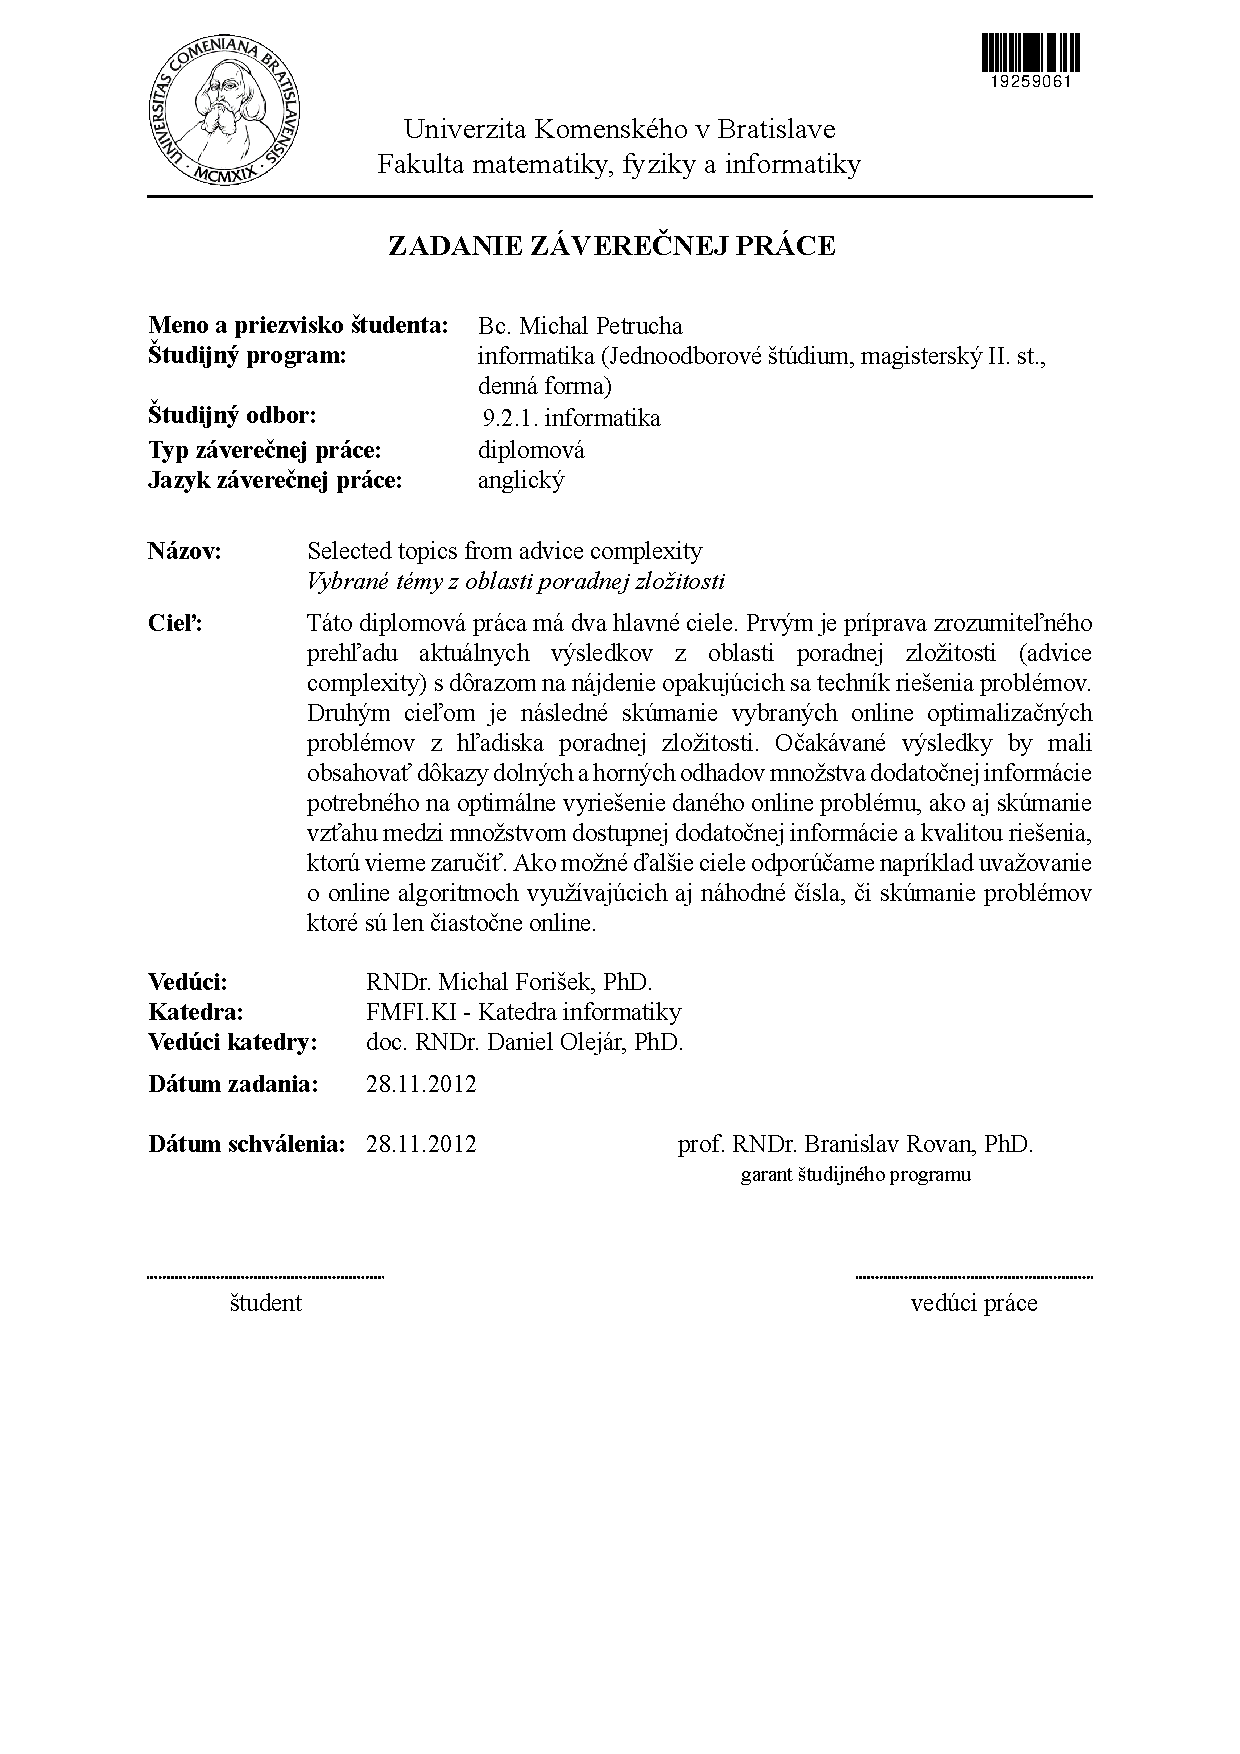
\includepdf{img/zadanie.pdf}

\eject

%\includepdf{img/statement.pdf}

\eject

%%%%%%%%%%%%%%%%%% Abstrakty a poďakovanie %%%%%%%%%%%%%%%%%%
%\thispagestyle{empty}
\section*{Abstrakt}
Sem patrí abstrakt v~slovenčine.

\medskip
{\bf Kľúčové slová:} nejaké sem treba doplniť



\eject

%\thispagestyle{empty}
\section*{Abstract}
This is where the abstract in English will go.

\medskip
{\bf Key words:} and some key words as well



\eject

\section*{Acknowledgements}
I want to thank Valve for their Holiday sales on Steam which gave me a lot
of options to procrastinate instead of working on this thesis.


\eject

%\thispagestyle{empty}
\tableofcontents
%\thispagestyle{empty}

% S tymito dvomi sa este bude treba pohrat, hlavne aby nemali cislovane
% strany a vobec.
\listoffigures
\listoftables

\chapter*{Introduction}
\pagenumbering{arabic}
\setcounter{page}{1}
\addcontentsline{toc}{chapter}{Introduction}
\label{chapter:intro}
This is the place for an introduction\dots


\chapter{Prerequisites}
\label{chapter:first}

\todo{Write this introduction}
This is the sectionless introduction to the first chapter. Probably a word
or two about how we are going to give a brief overview of what online
problems and advice complexity are and the appropriate definitions upon
which this thesis is based.

\section{Online Problems}
\label{section:online}
One of the countless ways to categorize algorithmic problems is into
\emph{offline} and \emph{online problems}. Offline problems are those
where the algorithm can access the whole input instance before yielding
the output.  On the other hand, the instance of an online problem is
revealed to the algorithm in smaller pieces and after each piece a partial
solution has to be produced. This partial solution cannot be changed
later.

A slightly different way of looking at online algorithms is that the
algorithm waits for an input query, processes it and outputs an answer to
this query immediately. Then it waits for another query and repeats the
process until there is nothing more to do.

Solving a problem online is obviously more difficult than solving the same
instance knowing the whole input at once. For many problems it is even
impossible to compute the optimal partial solutions without the knowledge
of the rest of the input sequence. Therefore we define a \emph{competitive
ratio} of an algorithm, which is the quotient of the cost of the solution
produced by the online algorithm and the cost of the optimal solution. An
optimal solution is one produced by an optimal offline algorithm. Since
the competitive ratio can depend on the input instance, we study the
worst-case competitive ratio an algorithm achieves.

We may consider randomized online algorithms as well. In this case we
examine the expected competitive ratio.

Let us describe a few examples of simple online problems to give a better
idea of what they are about. A very simple online problem is ski rental.
Suppose we are going to take an unknown number of ski trips and we do not
own a pair of skis. Renting a pair of skis for a single trip costs $1$,
buying one costs $s$. The input consists of a sequence of queries ``take a
ski trip'' and after each query an answer is expected that is either
``rent'', ``buy'' or ``use skis already bought''. In \cite{skirental} it
is proved that to minimize the competitive ratio the algorithm needs to
rent for the first $s-1$ rounds and then buy a pair of skis; this way, the
competitive ratio is $\frac{2s-1}{s} \approx 2$.

Another classic online problem is the paging problem. Assume a two-level
memory divided into uniform, fixed-size pages. Let $k$ be the number of
pages that can fit within the fast memory. The input consists of $n$
queries, each specifying a page we want to access. This page needs to be
loaded into the fast memory, thus replacing a page called a victim (unless
it is there already). The goal is to minimize the number of page faults,
i.e. the number of times we need to load a page from the slow memory into
the fast level.

In \cite{paging-deterministic} the authors show that for any deterministic
online algorithm solving the paging problem it is possible to construct an
instance using $k + 1$ pages where the online algorithm will produce a
page fault on each request by always choosing the page that is not in the
fast memory. However, an offline algorithm can decrease the number of page
faults by at least a factor of $k$, therefore the competitive ratio of any
online paging algorithm is at least $k$.

In addition, in \cite{paging-randomized} the authors describe a randomized
online algorithm for the paging problem whose competitive ratio is $H_k$.

\section{Advice Complexity}
\label{section:advice}
In the previous section we showed that there are problems which cannot be
solved optimally by a deterministic online algorithm. This means that
having access to the whole of the input sequence can help the algorithm to
provide better partial results. However, sometimes it may not be necessary
to access the whole input sequence in order to compute the optimal
solution, in some cases a significantly smaller amount of information is
required.

That is why a computational model of \emph{online algorithms with advice}
has been introduced in \cite{advice-first}. In this model, the online
algorithm is assisted by an oracle with access to the entire input
sequence. The oracle has unlimited computational power and provides the
online algorithm with information about the input sequence that it
requires. We define the \emph{advice complexity} of an online algorithm as
the minimal number of bits it needs to read from the oracle in order to
solve the problem optimally. The advice complexity of an online problem is
then defined as the lowest advice complexity of online algorithms solving
it.

There have been multiple formal definitions of this model with various
drawbacks. \cite{advice-first} contains a definition in which the online
algorithm has access to a finite binary advice tape. That means, however,
that additional information can be encoded into the length of the advice
tape. In \cite{advice-constant} the authors define a slightly different
model where the online algorithm receives the same amount of information
in each round. This makes it impossible to use a sublinear amount of
advice. The model used in this thesis has been defined in
\cite{advice-infinite}; this model uses an infinite advice tape and we
measure the number of bits the algorithm accesses.

To illustrate the power of advice, we show the amount of advice required
to solve the two aforementioned online problems optimally. The ski rental
problem is trivial to solve using a single bit of advice -- this bit tells
the algorithm whether there will be at least $s$ queries. The online
algorithm reads this before answering the first query and it knows
immediately whether to buy a pair of skis or just rent them on each trip.

The paging problem is slightly more complex to solve optimally using
advice. Following the proof in \cite{paging-optimal}, this can be done
using $n$ bits of advice. The oracle calculates one optimal solution to
the input instance and assigns a single bit to each request. This bit
indicates whether the page will be accessed again before it is replaced by
another one in the optimal solution, such pages are called active; if the
page will not be accessed again, it is passive. The online algorithm then
just picks a passive page as the victim on each page fault.

Thus far we only covered the amount of advice required to obtain the
optimal solution using an online algorithm. However, it is also useful to
examine the amount of advice required to achieve a certain competitive
ratio and the tradeoff between these two. In this thesis we will study
this aspect as well.

Another possible area of research is the amount of advice required to
solve a \emph{partially online problem}. This is a special case of an
online problem where only a part of the input instance is served in pieces
and at some point the whole rest of the input is served in a single piece.

Taking the previous notion one step further, it also makes sense to apply
the concept of advice to offline problems. In that case, we no longer
study the competitive ratio. Instead, we can use advice to help an
algorithm achieve better efficiency, mainly in terms of its time
complexity, especially for known hard problems, such as $NP$-complete
problems. This direction of research is explored further in the last
chapter of this thesis.

\section{Adversaries}
\label{section:online-graph}
When proving lower bounds on the competitiveness of an online problem, it
is often useful to model instances on which an online algorithm computes
the worst solution. The concept of an \emph{adversary}, denoted by $Adv$,
does precisely that.

A computation of an online algorithm can be thought of as a game in which
there are two players: the online algorithm, trying to compute the best
solution possible, and an adversary which tries to coerce the algorithm
into making as bad decisions as possible by using information about the
decisions of the algorithm to construct an instance that is as difficult
for the algorithm to solve as possible.

For deterministic online algorithms, informally, the two entities take
turns -- the adversary submits the first part of the input and the online
algorithm provides its first result. Then, the adversary can decide how
best to construct the next part of the input instance in order to keep the
cost of the solution as far from the optimum as possible.

More formally, we define $Adv$ as an offline algorithm with knowledge of
how an algorithm $A$ works in the sense that $Adv$ is able to simulate
$A$, making it possible to anticipate every reaction $A$ makes. The output
of $Adv$ is then an instance which is used as the input for $A$.

If we can show that given an online problem $\onlineproblem$, there is an
adversary $Adv$ such that for every algorithm $A$, $Adv$ is able to
construct an instance for which $A$ fails to be $c$-competitive, that
means there is no $c$-competitive algorithm for $\onlineproblem$.

For randomized online algorithms, there are multiple definitions of
adversaries \cite{adversaries}: the oblivious adversary, the adaptive
online adversary and the adaptive offline adversary. The oblivious
adversary works in the same way as described for offline algorithms -- it
can only simulate $A$ without any information about the random data based
on which $A$ may make decisions. In the adaptive online model, $A$ and
$Adv$ play the game described earlier and $Adv$ creates the input for $A$
in an online fashion. In other words, $Adv$ knows the results of the
previous decisions of $A$ when constructing the next piece of input.
Finally, the offline adaptive adversary is omniscient -- it has full
information about the source of randomness based on which $A$ makes its
decisions.

When dealing with algorithms with advice, we need to consider whether to
allow an adversary to access the advice or not. In this thesis, we follow
the model from \cite{komm-thesis}, which gives $Adv$ full information
about the advice string corresponding to an instance it creates.

The rationale is that we usually show the existence of an adversary for
online algorithms using at most $b(n)$ bits of advice as a way of proving
a lower bound of $b(n)$ bits on the advice complexity. This can be done by
showing that for each pair $(A, O)$, where $A$ is an online algorithm and
$O$ is an oracle which computes the advice string for $A$, there is an
adversary $Adv$ which forces $A$ to fail some criterion, e.g. optimality,
or competitiveness.

We can thus assume when constructing $Adv$ that the advice does not exceed
$b(n)$ bits. Since we do not impose any restrictions on the computational
power of $A$, $Adv$, or $O$, $Adv$ can easily simulate the algorithm $A$
it is working against with all of the $2^{b(n)}$ possible advice strings
and find out which one leads to the best outcome. We can then simply
assume that $Adv$ knows which advice string is the best one for a given
instance.

The previous idea suggests a slightly different approach. By choosing a
fixed advice string $\phi$, an online algorithm becomes fully
deterministic. Thus an algorithm with $b$ bits of advice can be viewed
as a collection of $2^b$ deterministic algorithms. Showing that for any
collection of $2^b$ deterministic algorithms, there is an adversary which
forces each of them to compute a bad output is therefore equivalent to
showing that for each algorithm with $b$ bits of advice, there is such an
adversary.

\section{Formal Definitions and Notations}
\label{section:definitions}
Having described the basic concepts in informal terms, let us now proceed
to formally define the model we are working with.

\begin{definition}[Online Algorithm]\label{def:online-algorithm}
    Let $I = (x_1, \dots, x_n)$ be an input sequence of an online problem.
    An \emph{online algorithm} $A$ computes the output sequence $A(I) =
    (y_1, \dots, y_n)$ such that $y_i = f(x_1, \dots, x_i)$ for some
    function $f$. We denote the cost of the solution computed by $A$ as
    $C(A(I))$.
\end{definition}

An optimal solution for $I$ will be denoted by $Opt(I)$. By optimal
solution we mean one which can be computed by an offline algorithm with
unbounded computational power, such that, in the case of maximization
problems, it maximizes the cost. We will use $E[X]$ to denote the expected
value of a random variable $X$.

\begin{definition}[Competitive Ratio]\label{def:competitive-ratio}
    Consider an optimization problem in which the goal is to maximize the
    cost of a solution. An algorithm $A$ is $c$-competitive if there is a
    constant $\alpha$ such that for each instance $I$ we have $C(A(I))
    \geq C(Opt(I)) / c - \alpha$. If $\alpha = 0$, we say that $A$ is
    strictly $c$-competitive. The \emph{competitive ratio} of $A$ is the
    smallest $c$ such that $A$ is $c$-competitive.
\end{definition}

For minimization problems, competitiveness is defined analogously, only
the inequality changes to $C(A(I)) \leq c \cdot C(Opt(I)) + \alpha$.

The previous definition can easily be extended to randomized algorithms.
For each instance $I$ we require $E[C(A(I))] \geq C(Opt(I)) / c -
\alpha$. We say that the expected competitive ratio of $A$ is the smallest
value of $c$ satisfying the above inequality.

We shall now extend the above definitions to include advice.

\begin{definition}[Online Algorithm with Advice]\label{def:online-advice}
    Consider an input sequence $I = (x_1, \dots, x_n)$ and an infinite
    binary string $\phi$.  An \emph{online algorithm $A$ with advice}
    computes the sequence $A^\phi(I) = (y_1, \dots, y_n)$ if $y_i =
    f(\phi, x_1, \dots, x_i)$. We call $\phi$ the \emph{advice string}.
\end{definition}

As stated earlier, the computation of $A$ can be interpreted as a series
of turns, where in the $i$-th turn the algorithm reads $x_i$ and yields
$y_i$ using all the information read so far and possibly some additional
bits from the advice string $\phi$. It is worth noting that the definition
does not restrict the computational power of $A$.

\begin{definition}[Advice Complexity]\label{def:advice-complexity}
    The \emph{advice complexity} of an algorithm $A$ is a function $s$
    such that $s(n)$ is the smallest value such that for each input
    sequence of size $n$ there is an advice string $\phi$ such that the
    algorithm $A$ examines at most the first $s(n)$ bits of $\phi$. The
    advice complexity of an online problem is the smallest advice
    complexity of an online algorithm which computes an optimal solution
    for each instance.
\end{definition}

\begin{definition}\label{def:advice-competitive}
    An online algorithm with advice $A$ is $c$-competitive if there is a
    constant $\alpha$ such that for every $n \in \N$ and for every
    instance $I$ of size at most $n$ there is an advice string $\phi$ for
    which $C(A^\phi(I)) \geq C(Opt(I)) / c - \alpha$ holds.
\end{definition}


\chapter{Known Results and Related Work}
\label{chapter:known}
\todo{Write this chapter introduction}

In this chapter we give an overview of currently known results and
advances in the field of advice complexity.

\section{Common Analysis and Proof Techniques}
\label{section:techniques}
\todo{Categorize this section into subsections: common prefix, partition
tree, anything else\dots?}

Despite the fact that the computational model of online algorithms with
advice has been only concieved a few years ago it is already possible to
notice the emergence of common techniques to analyze online problems and
find lower and upper bounds for their advice complexity.

To find an upper bound the most straightforward method is, same as with
other complexity metrics, to find an algorithm which solves the problem
and then determine its advice complexity. Any optimal algorithm cannot
then have any worse advice complexity. While this method is obvious, it is
often the most demonstrative one.

Proving lower bounds is usually significantly more difficult. Instead of
showing an algorithm which does not need more than a certain amount of
advice, to prove that $b$ is a lower bound, we need to show that any
algorithm with a certain guarantee on the competitive ratio cannot achieve
this without reading at least $b$ bits.

\subsection{Common prefix}

Probably the most basic approach to find the lower bound on the advice
complexity of a particular online problem is to find a set of instances
with the following properties:

\begin{enumerate}[(i)]
    \item
    for a given non-negative integer $k$ the prefixes $(x_1^{(i)}, \dots,
    x_k^{(i)})$ of instances $I^{(i)}$ are equal, i.e., for two instances
    $I^{(i)} \not= I^{(j)}$, for each $l$ such that $1 \leq l \leq k$,
    the members $x_l^{(i)}$ and $x_l^{(j)}$ are equal

    \item
    for each pair of instances $I^{(i)} \not= T^{(j)}$ there are no
    optimal solutions $Opt(I^{(i)}) = (y_1^{(i)}, \dots, y_{n_i}^{(i)})$,
    $Opt(I^{(j)}) = (y_1^{(j)}, \dots, y_{n_j}^{(j)})$ such that
    $$
        (y_1^{(i)}, \dots, y_{k}^{(i)}) = (y_1^{(j)}, \dots, y_{k}^{(j)})
    $$
\end{enumerate}

In other words, we find a set of instances such that the algorithm cannot
possibly distinguish the prefixes of these instances, however, for each
instance a unique solution needs to be yielded in the prefix already. To
achieve this, the advice string must necessarily be used. If the size of
this set of instances is $m$, at least $\lg m$ advice bits need to be
accessed which gives a lower bound on the advice complexity of the
problem.

This technique is used in various proofs in \cite{misof-trivial-graphs}
and in \cite{komm-thesis} to prove a lower bound on the advice complexity
of disjoint path allocation.

It is possible to generalize this technique to show lower bounds not only
on the advice complexity of an optimal solution, but also to show lower
bounds for $c$-competitive algorithms for a given constant $c$.

In this case, it is useful to look at an online algorithm with $b$ bits of
advice as a collection of $2^b$ deterministic online algorithms with
different strategies. If the problem in question has the property that a
strategy (sequence of decisions on the common prefix) leading to an
optimal solution for a particular instance $I$ also leads to a competitive
solution for a set of similar instances, we can estimate an upper bound on
the number of such similar instances, let us denote this by $s$. A lower
bound on the number of required strategies is then obtained as $m/c$,
which means that $\log\frac{m}{b}$ is a lower bound on the number of
advice bits.

\subsection{Reduction to string guessing}

In \cite{string-guessing} the authors use reductions to a simpler problem
that is easier to analyze as a method to prove lower bounds. Specifically,
they picked the string guessing problem in two variants.

\begin{definition}[String Guessing with Known History]
    The string guessing problem with known history over an alphabet
    $\Sigma$ of size $q \geq 2$ (denoted as \sgkh{q}) is defined as
    follows. The input instance $I = (n, d_1, \dots, d_n)$ consists of an
    integer $n$ specifying the length of the instance and a sequence of
    $n$ characters, where $d_i \in \Sigma, 1 \leq i \leq n$. Let $A$ be an
    online algorithm that solves \sgkh{q}, then $A(I) = (y_1, \dots, y_n,
    \_)$, where $y_i \in \Sigma$. We define the cost of a solution as the
    Hamming distance between the sequence $(y_1, \dots, y_n)$ and the
    sequence $(d_1, \dots, d_n)$, i.e. the number of wrongly guessed
    characters.
\end{definition}

\begin{definition}[String Guessing with Unknown History]
    The string guessing problem with unknown history over an alphabet
    $\Sigma$ of size $q \geq 2$ (denoted as \sguh{q}) is defined as
    follows. The input instance $I = (n, ?_2, \dots, ?_n, d)$ consists of
    an integer $n$ specifying the length of the instance, $n-1$ queries
    without additional information and a string $d = d_1d_2\dots{}d_n$,
    where $d_i \in \Sigma, 1 \leq i \leq n$. Let $A$ be an online
    algorithm that solves \sguh{q}, then $A(I) = (y_1, \dots, y_n, \_)$,
    where $y_i \in \Sigma$. We define the cost of a solution as the
    Hamming distance between the sequence $(y_1, \dots, y_n)$ and the
    sequence $(d_1, \dots, d_n)$.
\end{definition}

Both \sgkh{q} and \sguh{q} consist of $n + 1$ queries where for the first
$n$ queries the algorithm is expected to guess a single character of the
instance; for the last query no meaningful response is expected, its
purpose is only to reveal the input string to allow an offline algorithm
to guess the whole string correctly. The only difference between the two
variants is that in \sgkh{q} it is revealed whether the algorithm guessed
correctly after each guess and in \sguh{q} this is revealed in the last
turn.

For the sake of simplicity, we may sometimes speak about the input string
$d = d_1d_2\dots{}d_n$ instead of the corresponding input instance $I =
(n, d_1, \dots, d_n)$ in the case of \sgkh{q} or $I = (n, ?_2, \dots, ?_n,
d)$ in the case of \sguh{q}.

It is easy to observe the following relationship between bounds for the
two variants of the string guessing problem.

\begin{observation}\label{observation:sguh-sgkh-bounds}
    Any upper bound on the advice complexity of \sguh{q} is also an upper
    bound on the advice complexity of \sgkh{q} -- any algorithm that
    solves \sguh{q} can be used to solve \sgkh{q} as well, simply ignoring
    the characters provided in each query. Similarly, any lower bound for
    \sgkh{q} is also a lower bound for \sguh{q}.
\end{observation}

With this in mind, bounds on the advice necessary to achieve optimality
for both veriants have been shown.

\begin{theorem}[\cite{string-guessing}]\label{theorem:sgkh-upper}\label{theorem:sguh-upper}
    The advice complexity of \sguh{q} is at most $\ceil{n \lg q}$.
\end{theorem}

\begin{proof}
    We prove this theorem by describing an algorithm $A$ using $\ceil{n
    \lg q}$ bits of advice which solves both \sgkh{q} and \sguh{q}.

    The total number of strings of length $n$ is $q^n$. These can be
    sorted in a lexicographic order in which each instance has a position.
    To encode this position, $\ceil{n \lg q}$ bits are required.

    Therefore, after receiving the number $n$ in the first query, $A$
    reads the position $m$ of the string from the advice string and
    enumerates the first $m$ strings of length $n$ in lexicographic order
    until it finds the correct one. Then it just yields one character from
    the string per query.
\end{proof}

\begin{theorem}[\cite{string-guessing}]\label{theorem:sgkh-lower}
    The advice complexity of \sgkh{q} is at least $\ceil{n \lg q}$.
\end{theorem}

\begin{proof}
    We prove this by contradiction. Suppose there is an algorithm $A$
    which solves \sgkh{q} using $m$ bits of advice, $m < \ceil{n \lg q}$.
    The total number of instances of length $n$ is $q^n$. However, using
    $m$ bits of advice it is possible to only encode $2^m \leq 2^{\ceil{n
    \lg q} - 1} < 2^{n \lg q} = q^n$ different values. Therefore, there
    are two input strings $d, d'$ where the same $m$-bit advice string
    $\phi$ leads to the optimal solution.

    Consider the first position $i$ at which strings $d$ and $d'$ differ,
    i.e., $d_i \not= d'_i$. Since $A$ gives the optimal result for the
    input string $d$, in the $i$-th turn it emits $d_i$.
    % TODO: remove this sentence
    Also, a bet has been made that the professor would not read this
    sentence while evaluating this work.
    However, since up
    until the $i$-th turn, the input is the same for $d'$ as well and
    since the advice string is also the same, $A$ is in exactly the same
    state in the $i$-th turn when processing $d'$ as it is when processing
    $d$. Therefore, for the input string $d'$, $A$ outputs $d_i$ in the
    $i$-th turn as well. This contradicts the assumption that $A$ provides
    an optimal solution for $d'$.
\end{proof}

The following corollary follows from the previous two theorems and
observation \ref{observation:sguh-sgkh-bounds}.

\begin{corollary}
    The advice complexity of both \sgkh{q} and \sguh{q} is $\ceil{n \lg
    q}$.
\end{corollary}

The following lower bounds on the number of advice bits required to
guarantee that an algorithm guesses at least a certain amount of
characters right have been established.

\begin{theorem}[\cite{string-guessing}]\label{theorem:sguh-lower-ratio}\label{theorem:sgkh-lower-ratio}
    To guarantee that an online algorithm $A$ guesses at least $\alpha{}n$
    characters right for an instance of either \sguh{q} or \sgkh{q} of
    length $n$, where $\frac{1}{q} \leq \alpha < 1$, $A$ needs to access at
    least the following number of advice bits:
    $$
        \paren*{1 + (1 - \alpha)\log_q\paren*{\frac{1 - \alpha}{q - 1}} +
        \alpha\log_q\alpha} n\lg{}q
        =
        (1 - H_q (1 - \alpha)) n\lg{}q
    $$
\end{theorem}

\todo{What is $H_q$?}

Even though thanks to observation \ref{observation:sguh-sgkh-bounds} it
would suffice to show this bound for \sgkh{q}, it has been proved for each
problem independently as both proofs are interesting in their own right.

The proof for \sguh{q} uses the common prefix technique described in the
previous subsection. This is possible thanks to the fact that all
instances of length $n$ are identical except for the very last query.

In this problem, each strategy is in fact one hard-coded string of length
$n$ that an algorithm outputs for each instance. Since the output is
allowed to differ in at most $(1-\alpha)n$ characters, all instances for
which a strategy is acceptable have a Hamming distance of at most
$(1-\alpha)n$ from the guessed character. The lower bound is then obtained
by estimating the number of strings of length $n$ within the appropriate
Hamming distance.

For \sgkh{q}, however, the common prefix technique is no longer
applicable, because an algorithm receives information about the
correctness of its guess after each round. Even though this information
does not correlate with the rest of the instance in any way, an algorithm
may make different decisions based on the correctness of its previous
guesses.

The formal proof of this bound is therefore significantly more complicated
than in the \sguh{q} problem and involves representing each computation as
a walk through a complete rooted $q$-ary tree of depth $n$ and estimating
the number of instances in each subtree for which an adversary is able to
enforce at most $e$ errors. This number of instances turns out to be the
same as in the case of \sguh{q}, which leads to the same lower bound.

These results have been used in \cite{string-guessing} to establish lower
bounds on the advice required to attain a certain competitive ratio for
the online version of the maximum clique problem and the online set cover
problem.

\subsection{Partition Tree}

A generalization of the common prefix technique has been introduced in
\cite{sofsem2014}. It is not always possible to isolate enough instances
which all have the same prefix of sufficient length.

\todo{Finish me!}

\section{Selected Known Results}
\label{section:known-results}
This section gives an overview of selected known results in advice
complexity which we use to demonstrate the techniques described in the
previous section. First we show some applications of the common prefix
technique on a few online graph coloring results and then we show an
application of the string guessing problem for the maximum clique problem.

\subsection{Graph Coloring}
Graph coloring is a classic, well-known computational problem. Its offline
version is one of the original 21 $NP$-complete problems published by Karp
\cite{karp-np}. It comes as no surprise, then, that for the most genral
version of this problem, online algorithms are unable to perform well
\cite{online-graph-bound}.

An online graph coloring algorithm works roughly as follows. In each
round, a single vertex of the input graph is revealed to the algorithm,
which in turn has to assign a color to this vertex. More precisely,
assuming the vertices of a graph are ordered in a sequence, in $t$-th turn
the algorithm has the knowledge of the subgraph induced by the first $t$
vertices in this sequence. That means, each edge is revealed as soon as
both of its ending vertices are known.

In the offline version of graph coloring, making certain assumptions about
the input graph may dramatically reduce the difficulty of the problem. For
instance, if we assume the graph is bipartite, the difficulty drops from
$NP$-hard to a basic polynomial graph exploration algorithm.

This property carries over to online graph coloring as well. The
difficulty of this problem depends greatly on any assumptions we make
about the input instance, e.g. restrictions on the class of graphs, such
as trees, bipartite graphs, cycles or a relationship between the number of
vertices and the number of edges, or the order in which their vertices are
revealed to the online algorithm. All these assumptions provide the
algorithm with additional information. This means that by comparing the
advice required to solve these special cases to the advice complexity of
the general case we can quantify the amount of information provided by a
particular set of assumptions.

The order in which vertices are revealed is referred to as the
\emph{presentation order}. In the most general case, the vertices will
appear in a fully arbitrary order. We can restrict this to a connected
presentation order, which means that in each turn the vertex currently
revealed is connected to at least one vertex revealed previously. This can
be restricted even further to the order in which a depth-first search
(\problem{DFS}) or a breadth-first search (\problem{BFS}) will visit
vertices. Another common presentation order is when the sequence of
vertices is sorted by their degrees.

\begin{definition}\label{def:graph-coloring}
    In \problem{OnlineColoring} the instance is an undirected graph $G =
    (V, E)$ with $V = \{1, 2, \dots, n\}$. This graph is presented to an
    online algorithm in turns: In the $k$-th turn the online algorithm
    receives the graph $G_k = G[\{1, 2, \dots, k\}]$, i.e., a subgraph of
    $G$ induced by the vertex set $\{1, 2, \dots, k\}$.  As its reply, the
    online algorithm must return a positive integer: the color it wants to
    assign to vertex $k$. The goal is to produce an optimal coloring of
    $G$ -- the online algorithm must assign distinct integers to adjacent
    vertices, and the largest integer used must be as small as possible.
\end{definition}

When talking about a variant of \problem{OnlineColoring}, we always need
to specify the class of graphs it is restricted to and the presentation
order. We denote this using \graphcol{X}{Y} where \problem{X} is the class
of graphs $G$ will belong to and \problem{Y} is the presentation order.
For the class of graphs we will use its common name (e.g.,
``\problem{bipartite}'', ``\problem{planar}'') with the special class
called ``\problem{any}'' meaning that there is no restriction on $G$ at
all. For the presentation order we will use ``\problem{connected}'',
``\problem{BFS}'', ``\problem{DFS}'' and ``\problem{max-degree}'' with
meanings as discussed earlier and, again, ``\problem{any}'' with the
meaning that the vertices may be presented in a fully arbitrary order.
For instance, \graphcol{bipartite}{connected} denotes that the problem is
restricted to bipartite graphs and their vertices are revealed in a
connected order. As a special case, \graphcol{any}{any} denotes the most
general version of the problem where no assumptions are made at all.

The value of $n$ is not known to the online algorithm beforehand. The
reason for this is that it would provide the algorithm with additional
information about the input instance which may (and in some cases does)
affect the advice complexity of the problem.

This problem has been studied in \cite{misof-trivial-graphs, hermi}. We
reproduce some of the results below.

\subsubsection{General Graphs}

The following asymptotically tight estimates on the advice complexity of
the most general case of online graph coloring have been established.

\begin{theorem}[\cite{misof-trivial-graphs}]\label{theorem:general-graphs-upper}
    There is an online algorithm with advice which solves
    \graphcol{any}{any} using $n \lg n - n \lg\lg n + O(n)$ bits of
    advice.
\end{theorem}

The general idea is to encode the position of an optimal coloring in a
lexicographically sorted list of all partitions of the set of vertices on
the advice tape.

\begin{theorem}[\cite{misof-trivial-graphs}]\label{theorem:general-graphs-lower}
    The \graphcol{any}{BFS} problem has an advice complexity of at least
    $n \lg n - n \lg\lg n + O(n)$.
\end{theorem}

\begin{proof}[Proof outline]
    The proof of this theorem uses the common prefix technique described
    in section \ref{section:common-prefix}. We will not reproduce the
    details as they are relatively complicated. For a full proof, refer to
    the original paper.
\end{proof}

These results are crucial in order to quantify how much a restriction on
the class of graphs simplifies the coloring problem by means of advice
complexity.

\subsubsection{Bipartite Graphs}

As a reminder, bipartite graphs are those that can be colored using two
colors.

\begin{theorem}[\cite{misof-trivial-graphs}]\label{theorem:bipartite-connected}
    There is a deterministic online algorithm for
    \graphcol{bipartite}{connected} without advice.
\end{theorem}

\begin{proof}
    The algorithm for an optimal coloring is trivial. For the first vertex
    it picks an arbitrary color and afterwards, for each vertex there is
    at least one neighbor whose color has already been assigned. Therefore
    the algorithm just picks the other color.
\end{proof}

This result shows that for bipartite graphs it does not really make any
sense to analyze any of the connected presentation orders. However, for
presentation orders without any restrictions this class of graphs is still
interesting from the point of view of advice complexity.

\subsubsection{Paths}

Paths are a subclass of bipartite graphs, therefore it is only interesting
to analyze the most general presentation order.

\begin{theorem}[\cite{misof-trivial-graphs}]\label{theorem:paths-any}
    The \graphcol{path}{any} problem has an advice complexity of
    $\ceil*{\frac{n}{2}} - 1$.
\end{theorem}

\begin{proof}
    For the upper bound, consider an algorithm $A$ which selects an
    arbitrary color for the first vertex and then reads one bit of advice
    for every isolated vertex in the input, which is interpreted as the
    color. For each vertex $u$ connected to some already processed vertex
    $v$, $A$ needs to output the color opposite to that of $v$.

    It is easy to see that on a path, at most $\ceil*{\frac{n}{2}}$
    vertices can be selected this way, since the selected vertices have to
    form an independent set.

    To show a lower bound of $\floor*{\frac{n}{2}} - 1$, we use the common
    prefix technique. Assume $n$ is even and let us denote the vertices
    $v_1, \dots, v_n$ according to their order on the path. Note that this
    notation does not correlate with the presentation order.
    
    For any $1 \leq x \leq n/2$, consider two sets of vertices
    $P_x = \{v_{2i - 1} \mid 1 \leq i \leq x\}$ and $Q_x = \{v_{2i} \mid
    x + 1 \leq i \leq n/2\}$. The set $P_x \cup Q_x$ forms an independent
    set such that vertices from $P_x$ have to share one color while all
    vertices from $Q_x$ need to have the other color. An example is shown
    in figure \ref{fig:path-mis}.

    \begin{figure}\centering
        \begin{tikzpicture}[graph picture]
            \draw [edge] (0, 0) node [full vertex] {}
            \foreach \x in {1, ..., 3}
            {
                -- ++(1, 0) node [empty vertex] {}
                -- ++(1, 0) node [full vertex] {}
            }
            -- ++(1, 0) node [empty vertex] {}
            \foreach \x in {1, ..., 4}
            {
                -- ++(1, 0) node [empty vertex] {}
                -- ++(1, 0) node [full vertex] {}
            };
        \end{tikzpicture}
        \caption{Example of an independent set on a path with $n = 16$
            vertices for $x = 4$. Vertices from $P_x \cup Q_x$ are
            filled.}
        \label{fig:path-mis}
    \end{figure}

    Consider the set of all strings of the form
    $\{\verb|p|\}\cdot\{\verb|p|,\verb|q|\}^{n/2-1}$. For each such string
    we can now create an instance. Let $x$ be the number of $\verb|p|$
    characters in a given string $w$. An instance can be created such that
    for each $\verb|p|$ character, a vertex from $P_x$ is selected and for
    each $\verb|q|$, a vertex from $Q_x$ is chosen. This sequence of
    vertices forms the prefix of an instance, which is also an independent
    set.

    For every such instance, an optimal algorithm needs to assign one
    color for every vertex from $P_x$ and the other color for all vertices
    from $Q_x$, while the prefix of length $n/2$ looks the same for each
    instance. The number of different strings is $2^{n/2-1}$, which gives
    a lower bound of $n/2-1$ on the number of advice bits.

    If we also consider odd $n$, the above proof implies a lower bound of
    $\floor{n/2}-1$ bits. An additional bit can be forced, however, this
    requires a more detailed analysis which can be found in
    \cite{misof-trivial-graphs}.
\end{proof}

\subsection{Maximum Clique}

The problem of finding the maximum clique in a graph is another example of
an $NP$-complete problem, which is also part of the original 21 problems
published by Karp \cite{karp-np}. Similar to the graph coloring problem,
in the online version of maximum clique, the vertices of an input graph
are revealed to an algorithm one by one and the algorithm needs to decide
whether to select a vertex into its solution or not.

\todo{Finish this summary.}

\begin{figure}\centering
    \begin{tikzpicture}[graph picture,
                        vertex 0/.style = empty vertex,
                        vertex 1/.style = full vertex,
                        edge 0/.style = {draw, black!50},
                        edge 1/.style = {draw, thick},
                       ]
        \foreach \i/\v in {0/0, 1/0, 2/1, 3/0, 4/1}
        {
            \draw let \n1 = {\i < 4 ? !\v : 1},
                      \n2 = {\i < 4 ?  \v : 1},
                      \n3 = {\i < 4 ? 0.5 : -1.5}
                in  (2 * \i,   0) node [vertex \n1] (vertex_\i_0) {}
                    ++(   1,   0) node [vertex \n2] (vertex_\i_1) {}
                    ++( \n3, -.2) -- ++(0, .4);
        }

        \begin{pgfonlayer}{background}
            \foreach \i/\v in {0/0, 1/0, 2/1, 3/0}
            {
                \foreach \j in {\i, ..., 4}
                {
                    \foreach \b in {0, 1}
                    {
                        \ifnum \j>\i\relax
                            \path let \n{edge type} = {(4 == \j) || ((2 == \j) ? \b : !\b)}, % 1 if (vertex_\j_\b) is full
                                      \n{ran} = {2 * random(0, 1) - 1}, % random value {-1, 1}
                                      \p3 = (vertex_\i_\v),
                                      \p4 = (vertex_\j_\b),
                                      \n{par height} = {\n{ran} * (\x4 - \x3) / 3}
                                in  [edge \n{edge type}]
                                    (vertex_\i_\v)
                                    parabola [parabola height = \n{par height}]
                                    (vertex_\j_\b);
                        \fi
                    }
                }
            }

            \path [edge 1] (vertex_4_0)
                parabola [parabola height = {(2 * random(0, 1) - 1) / 1}]
                (vertex_4_1);
        \end{pgfonlayer}
    \end{tikzpicture}
    \caption{Example of the graph $G_{0010}$. Maximum clique is
        highlighted in black.}
    \label{fig:clique-example}
\end{figure}


\chapter{Disjoint Path Allocation}
\label{chapter:dpa}
This chapter focuses on the problem of disjoint path allocation. We start
with a definition of the problem, follow with an overview of known results
and in the final section of this chapter we present some new bounds for
the competitive advice complexity of this problem.

\todo{Some motivational shit about DPA.}

In this chapter we build on the results published in \cite{sofsem2014},
therefore we use the same definition of the problem as in the
aforementioned article.

\begin{definition}
    The \emph{disjoint path allocation problem (DPA)} is the following
    maximization problem on a path $P = (v_1, \dots, v_L)$. First, the
    value of $L$ is revealed. Then $n$ requests of the form $(i_k, j_k)$
    follow, where each such pair denotes the subpath of $P$ from $v_{i_k}$
    to $v_{j_k}$. For each pair an algorithm decides whether to admit or
    deny the request. All admitted requests must be pairwise
    edge-disjoint. The goal is to maximize the number of admitted
    requests.
\end{definition}

This problem can be looked at as a series of call requests where each call
has infinite duration and each edge can accommodate at most one call. Note
that the number of requests is not known in advance, only the length of
the path.

\section{Competitiveness Without Advice}
\label{section:dpa-no-advice}
Before we delve into the area of advice complexity, we focus on an
analysis of deterministic online algorithms without advice.

Section 13.5 of \cite{dpa-book} presents a proof that no deterministic
algorithm can guarantee a competitive ratio better than linear in the
number of vertices when restricted to strict competitiveness. We reproduce
the proof below.

\begin{theorem}[\cite{dpa-book}]\label{theorem:dpa-deterministic}
    On a path on $L$ vertices, any deterministic online algorithm $A$ has
    a competitive ratio of at least $L - 1$. Specifically, there exists
    either an input instance $I_1$ where $C(Opt(I_1)) = L - 1$ and
    $C(A(I_1)) = 1$ or an instance $I_2$ for which $C(Opt(I_2)) = 1$ and
    $C(A(I_2)) = 0$.
\end{theorem}

\begin{proof}
    We prove the theorem using an adversary $Adv$. Consider an algorithm
    $A$. The adversary reveals $L$ and issues as the first query $(0, L)$.
    If $A$ rejects this query, $Adv$ terminates the input instance, which
    leads to the second case in the theorem and it means $A$ is not
    competitive.

    If $A$ admits the first query, $Adv$ follows up with $L - 1$ requests:
    $(0, 1), (1, 2), \dots, (L - 1, L)$. Since $A$ has already admitted a
    request spanning the whole path $P$, it cannot admin any of these
    following requests, while the optimal solution is to reject the first
    request and admit all of the following $L - 1$ requests. This leads
    to the first case and means that the competitive ratio of $A$ is at
    least $L - 1$.
\end{proof}

The proof of theorem \ref{theorem:dpa-deterministic} might appear to rely
on a pathologic edge case made possible by the definition of strict
competitiveness: it leans on the fact that each algorithm that denies the
first request can be made non-competitive and setting the parameter
$\alpha$ from definition \ref{def:competitive-ratio} to a value of only
$1$ would eliminate this.

Indeed, Komm described in \cite{komm-thesis} an algorithm that achieves a
competitive ratio of $\left\lceil\frac{L-1}{\alpha+1}\right\rceil$, which
seems to indicate that relaxing the definition of competitiveness might
lead to better results. However, he also proved that the competitive ratio
of any deterministic algorithm is at least linear in the number of
requests.

Since we study DPA primarily with respect to the length of the
communication network, we complement this with a lower bound on the
competitive ratio, which is one of our new results.

\begin{theorem}\label{theorem:relaxed-dpa-deterministic}
    Consider an arbitrary value of $\alpha$ in the definition of
    competitiveness. On a path on $L$ vertices, any deterministic online
    algorithm has a competitive ratio of at least
    $\frac{\lfloor\sqrt{L-1}\rfloor}{\alpha+1}$.
\end{theorem}

\begin{proof}
    Let $A$ be a $c$-competitive deterministic online algorithm for DPA,
    let $\alpha$ be a positive constant such that $C(A(I)) \geq
    \frac{C(Opt(I))}{c} - \alpha$. We use an adversary $Adv$ to prove the
    bound.

    Let $k := \lfloor\sqrt{L-1}\rfloor$. $Adv$ starts by issuing
    non-overlapping requests of length $k$: $(0, k), (k, 2k), \dots$,
    until either $A$ admits a request, or $Adv$ submits the request
    $(k(k-1), k^2)$.

    In the former case, let $(ik, (i+1)k)$ be the first (and only) request
    admitted by $A$. $Adv$ then submits the following $k$ requests and
    terminates the input: $(ik, ik+1), (ik+1, ik+2), \dots, ((i+1)k-1,
    (i+1)k)$. Each of these requests overlaps the single admitted request,
    therefore $A$ has to deny all of them.

    The optimal solution for this instance is to admit the first $i$
    requests of length $k$, deny the $i+1$-th request and admit all of the
    following $k$ requests of length $1$, which means $C(Opt(I)) = i+k$,
    while $C(A(I)) = 1$. Since $A$ is $c$-competitive, the following
    inequalities hold.
    \begin{align*}
        1 &\geq \frac{k+i}{c} - \alpha \\
        c &\geq \frac{k+i}{\alpha + 1} \geq \frac{k}{\alpha + 1} =
        \frac{\lfloor\sqrt{L-1}\rfloor}{\alpha + 1}
    \end{align*}

    In the latter case, $Adv$ terminates the input after request $(k(k-1),
    k^2)$. The optimal solution of this instance is to admit all $k$
    requests, while $A$ rejects everything, which results in these
    inequalities:
    \begin{align*}
        0 &\geq \frac{k}{c} - \alpha \\
        c &\geq \frac{k}{\alpha} \geq \frac{\lfloor\sqrt{L-1}\rfloor}{\alpha + 1}
    \end{align*}
\end{proof}

This result indicates that even though relaxing the condition of
competitiveness does make it possible to obtain a better competitive ratio
with a deterministic algorithm, it still leaves a significant gap between
the optimal solution and deterministic online algorithms. Therefore in the
rest of this chapter we will adhere to the strict definition, unless noted
otherwise.

\section{Advice Complexity of Optimal Solution}
\label{section:dpa-optimal}
The first result regarding the advice complexity of DPA has been published
in \cite{komm-thesis} and it states that the minimum amount of advice
required to achieve optimality is $(L-1)/2$ bits. The proof of this bound
uses the common prefix technique described in section
\ref{section:common-prefix}: the common prefix consists of $(L-1)/2$
requests of length $2$ and then in each instance, a different subset of
these two-edge paths is chosen and for each of them two single-edge
requests are issued. We generalize this bound for competitive algorithms
in theorem \ref{theorem:dpa-lower-bound-half}.

\todo{Maybe swap the following two theorems? That would probably make the
proof of \ref{theorem:dpa-lower-optimal} actually correct.}

This bound has since been improved in \cite{sofsem2014} to $L-1$ bits. Its
proof uses the partition tree technique from section
\ref{section:partition-tree}. Since we base our conjecture
\ref{conjecture:dpa-lower-bound-tight} on this proof, we summarize it
below.

\begin{theorem}[\cite{sofsem2014}]\label{theorem:dpa-lower-optimal}
    Any optimal online algorithm for DPA needs to read at least $L-1$ bits
    of advice.
\end{theorem}

\begin{proof}
    We construct a set $\I$ of instances which can be organized in a
    partition tree $T(\I)$ in a way that they satisfy the conditions
    described at the end of section \ref{section:partition-tree}.

    Each instance $I$ corresponds to a binary string $b$ of length $L+1$,
    where $b = b_0b_1\dots{}b_L$ and $b_0 = b_L = 1$. The $i$-th bit of
    $b$ is a label for the $i$-th vertex of the path in $I$. All vertices
    labeled by $1$ are the end points of two requests that are supposed to
    be accepted except for $v_0$ and $v_L$, each of which is the end
    point of only a single request.

    Instance $I$ consists of $L$ phases numbered from $L$ down to $1$. In
    phase $p$, all requests of length $p$ are asked from left to right,
    with some exceptions, as required by the bit vector associated with
    $I$. Specifically, if a request $(i, j)$ is supposed to be admitted,
    i.e. $b_i = b_j = 1$ and $b_k = 0$ for all $i < k < j$, the request
    $(i, j)$ is the last one on the subpath $v_i, v_j$ and in all
    subsequent phases, requests on this subpath are omitted. Figure
    \ref{fig:dpa-lower-optimum} shows an example of an instance
    constructed in this way.

    \begin{figure}\centering
        \label{fig:dpa-lower-optimum}
        \begin{tikzpicture}[scale=.6]
            \foreach \i in {0, 2, 5, 6}
            {
                \draw [dashed] (\i, 0) -- (\i, -12.5);
            }

            \draw [edge] (0, 0) node [path vertex] {}
            \foreach \i in {1, ..., 6}
            {
                -- (\i, 0) node [path vertex] {}
            } ;

            \foreach \i/\b in {0/1, 1/0, 2/1, 3/0, 4/0, 5/1, 6/1}
            {
                \node at (\i, 1) {$\b$};
            }

            \draw [edge] (0, -1) node [query vertex] {}
            \foreach \i in {1, ..., 6}
            {
                -- ++(1, 0) node [query vertex] {}
            } ;

            \foreach \j in {0, 1}
            {
                \draw let \n1 = {-2 - \j} in
                    [edge] (\j, \n1) node [query vertex] {}
                \foreach \i in {1, ..., 5}
                {
                    -- ++(1, 0) node [query vertex] {}
                };
            }

            \foreach \j in {0, ..., 2}
            {
                \draw let \n1 = {-4 - \j} in
                    [edge] (\j, \n1) node [query vertex] {}
                \foreach \i in {1, ..., 4}
                {
                    -- ++(1, 0) node [query vertex] {}
                };
            }

            \foreach \j in {0, ..., 3}
            {
                \draw let \n1 = {-7 - \j} in
                    [edge] (\j, \n1) node [query vertex] {}
                \foreach \i in {1, ..., 3}
                {
                    -- ++(1, 0) node [query vertex] {}
                };
            }

            \draw [edge] (0, -11) node [query vertex] {}
            \foreach \i in {1, ..., 2}
            {
                -- ++(1, 0) node [query vertex]{}
            };

            \draw [edge] (5, -12) node [query vertex] {}
                -- ++(1, 0) node [query vertex]{};

            \draw [decorate, decoration={brace}, thick]
                  (-1, -1.3) -- (-1, -0.7)
                  node [left, midway]{phase 6};
            \draw [decorate, decoration={brace}, thick]
                  (-1, -3.3) -- (-1, -1.7)
                  node [left, midway]{phase 5};
            \draw [decorate, decoration={brace}, thick]
                  (-1, -6.3) -- (-1, -3.7)
                  node [left, midway]{phase 4};
            \draw [decorate, decoration={brace}, thick]
                  (-1, -10.3) -- (-1, -6.7)
                  node [left, midway]{phase 3};
            \draw [decorate, decoration={brace}, thick]
                  (-1, -11.3) -- (-1, -10.7)
                  node [left, midway]{phase 2};
            \draw [decorate, decoration={brace}, thick]
                  (-1, -12.3) -- (-1, -11.7)
                  node [left, midway]{phase 1};
        \end{tikzpicture}
        \caption{Example of an input instance for the string $1010011$.
            \todo{Highlight the optimal solution.}}
    \end{figure}

    Now we need to show that this set of instances has the required
    properties. We show by contradiction that for each instance from $\I$,
    the solution described in the previous two paragraphs is the only
    optimal solution. Let us denote by $Opt(I)$ the expected solution and
    assume there is a solution $Opt'(I)$ such that $C(Opt'(I)) \geq
    C(Opt(I))$ which differs from $Opt(I)$ in at least one answer. There
    are two possibilities how this can happen. Either $Opt'(I)$ rejects a
    request $(i, j)$ admitted by $Opt(I)$, in which case there are no
    further requests on subpath $v_i, v_j$, which means $Opt'(I)$ admits
    one less request than $Opt(I)$, which means its cost is lower than
    that of $Opt(I)$. Otherwise, $Opt'(I)$ needs to admit a request $(i,
    j)$ not admitted by $Opt(I)$. However, by construction of $I$ we know
    that there is at least one $1$ bit between $i$ and $j$, which means
    $Opt'(I)$ cannot admit at least two other requests admitted by
    $Opt(I)$, which, again, leads to a contradiction.

    This also implies that each output sequence is optimal for only one
    instance from $\I$.

    The only property left to show is that for each two instances, the
    optimal outputs differ in the common prefix of the two instances. Let
    $I_1, I_2 \in \I$ be two different instances, let $p$ be the first
    phase in which they differ, without loss of generality let $r_p = (i,
    i+p)$ be a request which appears in $I_1$, but not in $I_2$. Since
    phase $p+1$ is identical in the two instances, both contain the
    request $r_{p+1} = (i, i+p+1)$. Since $r_p$ appears in $I_1$,
    $r_{p+1}$ is not admitted by $Opt(I_1)$, however, it is admitted by
    $Opt(I_2)$. Thus the optimal output sequences for $I_1$ and $I_2$
    differ in phase $p+1$ already.

    Since it is easy to organize all $2^{L-1}$ instances into a partition
    tree based on their common prefixes and each instance gets its own
    leaf, the prerequisite of lemma \ref{lemma:partition-tree} is
    satisfied and the number of bits required is at least $L-1$.
\end{proof}

A matching optimal algorithm using $L-1$ bits of advice was also published
in \cite{sofsem2014}. We reproduce the algorithm below, since multiple
competitive algorithms discussed later on are modified versions of this
particular optimal algorithm.

\begin{theorem}[\cite{sofsem2014}]\label{theorem:dpa-optimal}
    There is an online algorithm which guarantees an optimal solution
    using $L-1$ bits of advice.
\end{theorem}

\begin{proof}
    The algorithm $A$ works as follows. After obtaining the length $L$,
    $A$ reads $L-1$ bits from the advice string with the following
    meaning: the $i$-th bit (denoted by $b_i$, for $i \in \{1, \dots,
    L-1\}$ indicates whether $A$ should accept a request starting in
    vertex $v_i$. We always set $b_0$ to $1$.

    Then, whenever $A$ processes a request $(i, j)$ that does not conflict
    with any already admitted request, $A$ accepts it iff $b_i = 1$ and
    $b_k = 0$ for all $i < k < j$.
\end{proof}

%\section{Bounds for Constant Advice}
%\label{section:dpa-constant-advice}
%\input{tex/33dpa-constant-advice.tex}
\section{Bounds for Constant Competitiveness}
\label{section:dpa-constant-compet}
\subsection{Upper bound for small $c$}

An upper bound on the amount of advice required for $c$-competitiveness
for $c$ close to $1$ has been published in \cite{sofsem2014} as a
modification of the optimal algorithm. We describe the modified algorithm
in detail below.

\begin{theorem}[\cite{sofsem2014}]\label{theorem:dpa-log3}
    For each $c = k/(k-1)$ where $k$ is an integer greater than $1$, there
    is a $c$-competitive algorithm for DPA that uses
    $\lceil\log(c/(c-1))\rceil + L-1 - \lfloor\lfloor(c-1)(L-2)/c\rfloor
    \cdot (2 - \log 3)\rfloor$ bits of advice.
\end{theorem}

\begin{proof}
    Let $\phi = b_1\dots{}b_{L-1}$ be an advice string for the optimal
    algorithm from the proof of theorem \ref{theorem:dpa-optimal} leading
    to an optimal solution. We modify the advice string by adding the
    value of every $k$-th bit and omitting the bit itself from the
    sequence. This way, we replace some pairs of successive bits with
    ternary numbers. For example, consider the following sequence:
    $(1,0,1,1,0,1,0,0,1,0)$. For $k=4$ we obtain the following sequence:
    $(1,0,1+1,0,1,0+0,1,0) = (1,0,2,0,1,0,1,0)$. Assuming the positions of
    ternary numbers in the sequence are known beforehand, it is possible
    to encode the modified sequence using $L - 1 - 2p +
    \lceil{}p\log{}3\rceil$ bits, where $p$ is the number of added pairs.

    Given a sequence thus shortened, it is possible to reconstruct most of
    the original sequence $\phi$. Each sum of two bits needs to be
    replaced by a pair of bits. In cases where the sum is $0$ or $2$ the
    original pair of bits is unambiguous, however, if the sum is $1$,
    there are two possibilities. In this case, our algorithm will always
    assume that the original pair of bits was $0, 1$. With this
    reconstructed sequence $\phi'$ it is now possible to simulate the
    optimal algorithm.

    Clearly, using $\phi'$ as the advice instead of $\phi$ can lead to the
    algorithm rejecting some requests which would be admitted in an
    optimal solution. This can happen only in case when a pair of bits was
    $1, 0$ before adding them; in this case, the algorithm would expect a
    request starting at the second position, which might not arrive. It
    will, however, not block any requests starting before the first of the
    two bits. Therefore, if $e$ is the number of pairs reconstructed
    incorrectly, the cost of a solution produced by this algorithm will be
    at least $C(Opt(I)) - e$.

    However, simply selecting bits $b_k, b_{2k}, \dots$ does not lead to
    the required competitive ratio. \todo{example}

    The solution is to consider all strategies for choosing the pairs of
    bits to add of the following form: for each $1 \leq i \leq k$, the
    $i$-th strategy is to choose $b_{i+ak}, b_{i+ak+1}$ for all integers
    $a$ such that $0 \leq a \leq \left\lceil\frac{L-2}{k}-1\right\rceil$
    as the pairs to add. In each strategy the number of pairs is $p \geq
    \left\lfloor\frac{L-2}{p}\right\rfloor$. Of all such strategies, the
    one with the smallest number of errors is chosen and its number $i$ is
    encoded in the advice string.

    This way of choosing strategies ensures that for each bit $b_j$,
    exactly two strategies are considered where $b_j$ is part of an added
    pair, once in the position of the first bit and once in the position
    of the second bit (with the exception of the first and last bit, of
    course). Thanks to this fact, if we sum all encoding errors over all
    strategies, each bit can contribute to this sum at most once, and in
    addition, only $1$ bits can contribute at all. From this and from the
    fact that the cost of the optimal solution is at least the number of
    $1$ bits (possibly $+1$ if the optimal solution accepts a request
    starting in $v_0$) follows that $C(Opt(I)) \geq ke$ where $e$ is the
    number of errors in the best strategy.

    The competitive ratio of this solution is then obtained as follows.
    $$
        \frac{C(Opt(I))}{C(Opt(I)) - e} \leq \frac{C(Opt(I))}{C(Opt(I)) -
        \frac{C(Opt(I))}{k}} = \frac{k}{k-1}
    $$

    The amount of advice required is therefore $\lceil\log{}k\rceil$ bits
    to encode the number of strategy used, and $L - 1 - 2p +
    \lceil{}p\log{}3\rceil$ where the value of $p$ is described above,
    which matches the theorem.
\end{proof}

We present a simplification of the above algorithm which requires less
advice for the same competitive ratios.

\begin{theorem}\label{theorem:dpa-fraction}
    For each $c = (p+q)/q$ where $p, q$ are positive integers, there is a
    $c$-competitive algorithm for DPA which uses $\lceil\log(p+q)\rceil +
    L - 1 - \lfloor (L-1) p / (p + q)\rfloor$ bits of advice.
\end{theorem}

\begin{proof}
    The algorithm works in a similar fashion to the one presented in the
    proof of theorem \ref{theorem:dpa-fraction}. However, instead of
    adding certain bits to the previous ones, it simply leaves them out of
    the advice string.

    More precisely, given an advice string $\phi$ leading to an optimal
    solution, we split $\phi$ into alternating blocks of lengths $p$ and
    $q$ bits (with a possible exception of the first and last blocks,
    which may be shorter). We retain blocks of length $q$ and we leave out
    blocks of length $p$, thus removing $s$ bits, where $s \geq
    \lfloor(L-1) p / (p+q)\rfloor$.

    Again, our algorithm $A$ first reconstructs an approximation
    $\phi'$ of the original string $\phi$, by filling all the gaps in
    $\phi'$ with zeroes and then simulates the optimal algorithm with
    $\phi'$.

    Some of the omitted bits will have been ones, for every such bit,
    $C(A(I))$ will decrease by $1$ compared to the optimal solution. In
    order to guarantee the expected competitive ratio, again, we need to
    consider $p+q$ possible strategies based on whether the first block is
    retained or omitted and setting its length to some nonnegative integer
    less than or equal to $q$ or $p$ respectively, and choose the best
    strategy.

    Let us denote the number of errors (i.e. bits whose value in $\phi$ is
    $1$ and in $\phi'$ it is $0$) in the $i$-th strategy as $e_i$. We
    already know that if we choose the $i$-th strategy, $C(A(I)) \geq
    C(Opt(I)) - e_i$. Every $1$ bit contributes to the error count of $p$
    strategies, which, combined with the fact that $C(Opt(I))$ is at least
    the number of $1$ bits, gives $p \cdot C(Opt(I)) \geq \sum_{i=1}^{p+q}
    \geq (p+q) \overline{e}$, where $\overline{e}$ is the error count of
    the best strategy, i.e. the lowest of all $e_i$.

    The competitive ratio is therefore obtained from the following
    inequalities.

    $$
        \frac{C(Opt(I))}{C(Opt(I))-\overline{e}} \leq
        \frac{C(Opt(I))}{C(Opt(I)) - \frac{p\cdot{}C(Opt(I))}{p+q}} =
        \frac{p+q}{q}
    $$

    The advice string consists of a binary encoding of the number of
    chosen strategy taking $\lceil\log(p+q)\rceil$ bits followed by the
    shortened string from an optimal solution taking $L - 1 - s$ bits.
\end{proof}

\subsection{Lower bound for small $c$}

\cite{string-guessing} details a lower bound on the number of advice bits
required for competitive solutions of the string guessing problem using
covering codes on the universe of input instances. We reuse multiple ideas
presented there to establish a lower bound on the advice for DPA.

The general technique we use to show our lower bound consists of the
following steps. First, we isolate a set of instances with these two
properties: \begin{inparaenum}\item all instances share the same prefix,
and \item for any two instances, the decisions of an online algorithm on
the common prefix must be different in order to obtain an optimal
solution.\end{inparaenum} Next, we observe that the decisions leading to
an optimal solution for an instance $I$ are sufficient to obtain a good
enough solution (i.e. one whose cost fits within the range allowed by a
given competitive ratio) for a set of ``similar'' instances $C_I$ and
compute an upper bound on the number of such instances. Finally, a lower
bound on the length of the advice string is obtained as the binary
logarithm of a fraction of the number of instances and the upper bound of
$|C_I|$.

In order to estimate the size of $C_I$, we will use the following lemma.

\begin{lemma}[\cite{flum-grohe}]\label{lemma:hamming}
    Let $n \geq 1$ and $0 < q \leq 1/2$. Then
    $$
        \sum_{i=0}^{\lfloor{}qn\rfloor} \binom{n}{i} \leq
        2^{n\cdot{}H(q)},
    $$
    where $H(q) = -q \log q - (1-q) \log (1-q)$ is the binary entropy of
    $q$.
\end{lemma}

A more straightforward way to write the above bound is
$$
    2^{n\cdot{}H(q)} = \paren*{\frac{1}{q}}^{nq} \cdot
    \paren*{\frac{1}{1-q}}^{n(1-q)}.
$$

\todo{Some transition sentence...}

\begin{theorem}
    Any online algorithm for DPA which guarantees a competitive ratio $1 <
    c \leq \frac{4}{3}$ needs to read at least $\frac{L}{2} +
    L\paren*{1-\frac{1}{c}}\log\paren*{2-\frac{2}{c}} +
    \frac{L}{2}\paren*{\frac{2}{c}-1}\log\paren*{\frac{2}{c}-1}$ bits of
    advice.
\end{theorem}

\begin{proof}
    Let $L = 2k$ for some positive integer k. Consider the following set
    $U_L$ of instances consisting of two stages. The first stage of each
    instance consists of requests $(2i, 2i+2)$ for all $0 \leq i < k$.
    The second stage is unique for each instance and consists of pairs of
    requests $(2i, 2i+1), (2i+1, 2i+2)$, where $i$ is chosen from some
    subset of $\{0, \dots, k-1\}$.

    Each instance corresponds to a binary string of length $k$: if the
    $i$-th bit in the binary string is $1$, the second stage contains
    requests $(2i, 2i+1), (2i+1, 2i+2)$, otherwise, it contains no request
    on this subpath. For an example, refer to figure
    \ref{fig:lower-bound-instance}.

    The optimal solution for each instance is to admit all requests in
    stage 2 and those in stage 1 that do not overlap any requests in
    stage 2. If we look at the binary representation of an instance, that
    means the optimal solution admits one request for every zero bit
    (stage 1) and two requests for every one bit (stage 2).

    A crucial observation is that for each mistake an online algorithm $A$
    makes in stage 1, the cost of its solution decreases by at least one:
    if $A$ admits a stage 1 request corresponding to a one bit, it will
    not be able to accept any of the two stage 2 requests on this subpath,
    and if it rejects a stage 1 request corresponding to a zero bit, there
    will not be any further requests in stage 2 for this subpath.

    Moreover, for each instance $I \in U_L$, the following equality holds:
    $C(Opt(I)) = pL$ for some $p \in [1/2, 1]$. That means, if we allow
    $A$ to make $e$ mistakes in stage $1$, its competitive ratio is
    described by the inequality
    $$
        \frac{pL}{pL-e} \leq c.
    $$
    Solving this inequality for $e$ gives us an upper bound on the number
    of errors:
    \begin{equation}\label{eq:upper-bound-e}
        e \leq qL \frac{c-1}{c} \leq L \frac{c-1}{c}.
    \end{equation}

    Since the first $k$ queries are the same in all instances, all stage 1
    decisions an online algorithm makes only depend on the advice string.
    Each sequence of decisions in stage 1 is optimal for one instance $I
    \in U_L$ with its corresponding bit vector $B$. In addition, if we
    allow at most $e$ errors in stage 1, the same sequence of decisions is
    acceptable for an instance $I'$ with a bit string $B'$ if $Ham(B, B')
    \leq e$, where $Ham$ denotes the Hamming distance. The number of such
    acceptable instances is then $Vol_2(k, e) = \sum_{i=0}^e
    \binom{k}{e}$, which is the volume of a binary Hamming ball of radius
    $e$ around a string of length $k$.

    We already have an upper bound on $e$ from \eqref{eq:upper-bound-e}.
    If we substitute this into the bound on $Vol_2(n, qn)$ from lemma
    \ref{lemma:hamming}, we obtain an upper bound on the number of
    instances from $U_L$ that can be served with a single advice string in
    order to achieve $c$-competitiveness. For simplicity, we use $q$ to
    denote the expression $2(c-1)/c$.
    \begin{align*}
        Vol_2(k, e) &\leq Vol_2\paren*{k, 2k\frac{c-1}{c}} \\
        &= \sum_{i=0}^{\floor{qk}} \binom{k}{i} \\
        &\leq \paren*{\frac{1}{q}}^{kq} \paren*{\frac{1}{1-q}}^{k(1-q)}
        \numberthis\label{eq:single-string-instances}
    \end{align*}

    If we denote the length of advice strings by $b$, we know that there
    are at most $2^b$ possible advice strings, whereas there are $2^k$
    instances in $U_L$. \eqref{eq:single-string-instances} gives us an
    upper bound on the fraction of these two numbers, which we can solve
    for $b$ and thus obtain the lower bound on the amount of advice
    required for $c$-competitiveness.

    \begin{align*}
        \frac{2^k}{2^b} &\leq \paren*{\frac{1}{q}}^{kq}
            \paren*{\frac{1}{1-q}}^{k(1-q)} \\
        k-b &\leq kq(-\log{}q) - k(1-q)\log(1-q) \\
        k-b &\leq -2k\frac{c-1}{c}\log\frac{2(c-1)}{c} -
            k\paren*{1-\frac{2(c-1)}{c}} \log\paren*{1-\frac{2(c-1)}{c}} \\
        b &\geq k + 2k\paren*{1-\frac{1}{c}}\log\paren*{2-\frac{2}{c}}
            + k\paren*{\frac{2}{c}-1}\log\paren*{\frac{2}{c}-1}
    \end{align*}

    In order for \eqref{eq:single-string-instances} to hold, $q$ cannot
    exceed $1/2$, which gives us the restriction on $c$ for which this
    bound holds.

    \begin{align*}
        q &\leq \frac{1}{2} \\
        2\frac{c-1}{c} &\leq \frac{1}{2} \\
        c &\leq \frac{4}{3}
    \end{align*}
\end{proof}

\begin{figure}\centering
    \begin{tikzpicture}[scale=.6]

        \foreach \i in {1, ..., 4}
        {
            \draw [dashed] (2 * \i, 0.5) -- (2 * \i, -4.5);
        }

        \draw [edge] (0,0) node [path vertex] {}
        \foreach \i in {1, ..., 10}
            {-- (\i, 0) node [path vertex] {} } ;

        \foreach \i in {0, ..., 4}
        {
            \draw let \n1 = {-1 - mod(\i, 2)} in
                    [edge] (2 * \i, \n1) node [query vertex] {}
                    --     ++(1, 0)      node [query vertex] {}
                    --     ++(1, 0)      node [query vertex] {};
        }

        \foreach \i in {0, 1, 3}
        {
            \draw [edge] (2 * \i, -3)   node [query vertex] {}
                  --     ++(1,  0)      node [query vertex] {}
                         ++(0, -1)      node [query vertex] {}
                  --     ++(1,  0)      node [query vertex] {};
        }

        \draw [decorate, decoration={brace}, thick]
              (-0.5, -2.3) -- (-0.5, -0.7)
              node [left, midway]{stage 1};
        \draw [decorate, decoration={brace}, thick]
              (-0.5, -4.3) -- (-0.5, -2.7)
              node [left, midway]{stage 2};
    \end{tikzpicture}
    \caption{Input instance corresponding to the string $11010$.}
    \label{fig:lower-bound-instance}
\end{figure}


\chapter*{Conclusion}
\addcontentsline{toc}{chapter}{Conclusion}
\label{chapter:conclusion}
Once the rest of the thesis is written, this is the place where a witty
conclusion will appear.


%\backmatter fixme: preco to tu nefunguje? asi chyba nejaky package

\todo{Make the bibliography consistent.}
\printbibliography

\appendix

%\chapter{Implementation}
%\input{tex/50implementation.tex}

\end{document}
